\documentclass{article}

\usepackage[widepage]{repsty}
\usepackage{subcaption}

\newcommand{\W}{\Omega}
\newcommand{\w}{\omega}
\newcommand{\MDM}{{}^\mathrm{MDM}}
\newcommand{\EDM}{{}^\mathrm{EDM}}
\newcommand{\CW}{{}^\mathrm{CW}}
\newcommand{\CCW}{{}^\mathrm{CCW}}
\newcommand{\st}{\nu_s}



\begin{document}
\title{The Frozen Spin and Quasi-Frozen Spin lattice concepts}
There exist two design approaches to the problem of measuring the deuteron Electric Dipole Moment (dEDM) inside a storage ring: the Frozen Spin (FS) lattice, and the Quasi-Frozen Spin (QFS) lattice.

The FS ring design concept's main objective is the maximization of the EDM signal. In the case of a single particle, this can be accomplished if its spin is continuously aligned with the momentum vector in the horizontal plane: the so-called Frozen Spin condition. The continuous fullfilment of this condition, required by the FS method, is problematic for the following reasons:
\begin{itemize}
\item since the spin precession frequency $\vec\W = -\frac{q}{m}\bkt*{G\vec B + \bkt{\frac{1}{\gamma^2-1}-G}\vec\beta\times\vec E}$,~\cite{JEDI:SpinTuneMapping} the EDM of particles with a negative magnetic anomaly $G = (g-2)/2$ (such as the deuteron) cannot be measured using either a purely electrostatic or a purely magnetic ring, and so requires the use of combined E+B field elements, placed inside the accelerator arcs;
\item even so, for the given values of E- and B-fields, there exists a unique $\gamma$, for which the FS condition holds strictly, meaning that for the majority of the beam particles that condition is fulfilled only approximately in any case.
\end{itemize}
This last point is the major motivation for the use of a Quasi-Frozen Spin ring design.

The Quasi-Frozen Spin design concept consists in correcting the necessarily occurring MDM spin rotation in the magnetic arcs by a reverse rotation in the straight sections. The ring can be implemented in two versions: one in which the E- and B-field elements are separated, and another in which the combined E+B elements are located in the straight sections of the lattice.~\cite{Senichev:Shanghai}

In the first option, the ring is made up of two types of arcs: magnetic, in each of which the closed orbit is bent by an angle $\Phi^B_{co} = \pi + 2\alpha$, and the spin is rotated, accordingly, by $\Phi^B_{spin} = \st^B\cdot \Phi^B_{co}$, and electrostatic, with the closed orbit bend angle $\Phi^E_{co} = -2\alpha$, and $\Phi^E_{spin} = \st^E\cdot \Phi^E_{co}$. The Quasi-Frozen Spin condition in this case can be formulated simply as $\Phi^E_{spin} + \Phi^B_{spin} = 0$. One drawback of this lattice is the use of cylindrical electrostatic deflectors, and the non-linearities involved.

In the second option, straight E+B spin rotators (placed in the straight sections) are used to compensate the arc MDM rotation. 

If the spin vector oscillates in the horizontal plane with an amplitude $\Phi$, the EDM signal is reduced by a factor $1 - \frac{\Phi^2}{4}$. In a QFS ring with $n$-periodicity, the spin oscillates relative to the momentum vector within half the value of the advanced spin phase $\gamma G \cdot \frac{\pi}{2n}$.~\cite{Senichev:Shanghai} In our designs, with the accelerator length approximately 150 meters, $\Phi\approx 0.25$, and hence the signal is reduced by no more than 2\%.

\begin{figure}[h]
  \centering
  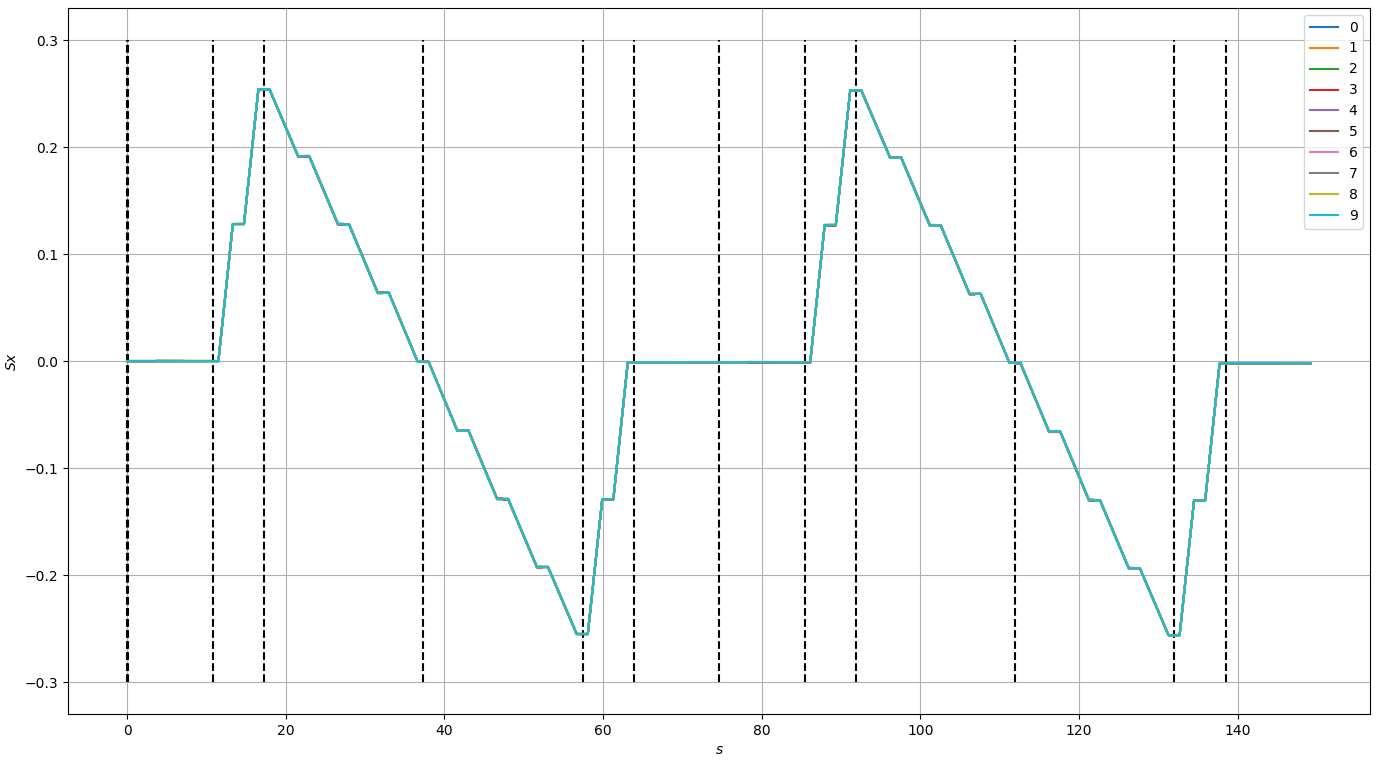
\includegraphics[width=\textwidth]{img/EB_QFS_Sx_vs_s_1turn}
  \caption{Spin precession in the horizontal plane in a QFS lattice. Dashed vertical lines mark the ends of sections of the lattice.\label{fig:QFS_Sx_vs_s}}
\end{figure}


\begin{thebibliography}{99}
\bibitem{JEDI:SpinTuneMapping}
  Saleev A, Nikolaev NN, Rathmann F, Augustyniak W, Bagdasarian Z, Bai M, et al. Spin tune mapping as a novel tool to probe the spin dynamics in storage rings. Physical Review Accelerators and Beams [Internet]. 2017 Jul 7 [cited 2018 Oct 8];20(7). Available from: \url{http://arxiv.org/abs/1703.01295}
  
\bibitem{Senichev:Shanghai}
  Senichev Y, Andrianov S, Ivanov A, Chekmenev S, Berz M, Valetov E 2015 Investigation of lattice for deuteron EDM ring. Proc. ICAP2015 (Shanghai, China). \url{http://accelconf.web.cern.ch/AccelConf/ICAP2015/papers/modbc4.pdf}

\bibitem{BNL_proposal}
  D. Anastassopoulos, V. Anastassopoulos, D. Babusci. AGS Proposal: Search for a permanent electric dipole moment of the deuteron nucleus at the $10^{−29} ~ e\cdot cm$ level. [Internet]. BNL; 2008 [cited 2016 Nov 25]. Available from: \url{https://www.bnl.gov/edm/files/pdf/deuteron_proposal_080423_final.pdf}
\bibitem{Mane:SpinWheel}
  S. R. Mane. Spin Wheel. arXiv:150901167 [physics] [Internet]. 2015 Sep 3 [cited 2018 Sep 28]; Available from: http://arxiv.org/abs/1509.01167
\bibitem{Senichev:FDM}
  Frequency domain method of the search for the deuteron electric dipole moment in a storage ring with imperfections

\bibitem{Senichev:StorageRingMethod}
  Yurij Senichev. Search for the Charged Particle Electric Dipole Moments in Storage Rings. In: 25th Russian Particle Accelerator Conference (RuPAC’16), St Petersburg, Russia, November 21-25, 2016 [Internet]. JACOW, Geneva, Switzerland; 2017 [cited 2017 Apr 5]. p. 6–10. Available from: \url{http://accelconf.web.cern.ch/AccelConf/rupac2016/papers/mozmh03.pdf}

\bibitem{Senichev:Decoh}
  Senichev Y, Zyuzin D. SPIN TUNE DECOHERENCE EFFECTS IN ELECTRO- AND  MAGNETOSTATIC STRUCTURES. In: Beam Dynamics and Electromagnetic Fields [Internet]. Changhai, China: JACoW; 2013 [cited 2017 Jul 31]. p. 2579--2581. Available from: \url{https://accelconf.web.cern.ch/accelconf/IPAC2013/papers/wepea036.pdf}

\end{thebibliography}
\end{document}
